\section{Second Problem}

\subsection{Problem Statement}

Fig\ref{problem 2} represents a double pendulum that is suspended from a block that moves
horizontally with a prescribed motion, $x(t)$: 
Derive the Euler-Lagrange equations of
motion of the pendulum when it oscillates in the $x-y$ plane under the action of gravity
and prescribed motion.

\begin{figure}[H]
    \centering
    \includegraphics[width=0.4\textwidth]{image/fig1.png}
    \caption{problem 2}
    \label{problem 2}
\end{figure}

\subsection{Hamilton's principle}

Hamilton's principle is one of the most fundamental principles in vibration analysis. 
It leads to the basic equations of dynamics and elasticity. It is based on the assumption that when a system moves from a state at a time 
$t_1$ to a new state at the time $t_2$. 
In a Newtonian route, 
then the actual route out of all the possible ones obeys stationarity. 
This condition leads to Hamilton's principle:
\begin{equation}
    \delta\int_{t_1}^{t_2}(T-V)dt=\delta\int_{t_1}^{t_2}Ldt = 0
\end{equation}

where $T$ is the kinetic energy of the system and $V$ is the potential energy of the system. 
Here $L$ represents:
\begin{equation}
    L=L(t,q_j,\dot{q}_j)
\end{equation}

where $q_j$ represents a freedom and $\dot{q}_j=\frac{d q_j}{dt}$ . Denote $H$ as:
\begin{equation}
    \delta H = \int_{t_1}^{t_2} \delta L dt
\end{equation}

thus we have:
\begin{equation}
    \delta H=
    \int_{t_1}^{t_2}
    \sum_{j=1}^N\left(
      \frac{\partial L}{\partial q_j}\delta q_j
      +
      \frac{\partial L}{\partial \dot{q}_j}\delta \dot{q}_j  
    \right)
    dt=0
\end{equation}

here $\delta \dot{q}_j$ represents a variation of $\dot{q}_j$:
\begin{equation}
    \int_{t_1}^{t_2}
    \delta \dot{q}_j dt=
    \delta q_j|_{t_1}^{t_2} = 0-0
\end{equation}

use integrate by part we will have:
\begin{equation}
    \begin{aligned}
        \int_{t_1}^{t_2}
    \frac{\partial L}{\partial \dot{q}_j}\delta \dot{q}_j dt
    &=
    \left.
    \frac{\partial L}{\partial \dot{q}_j}\delta q_j
    \right|_{t_1}^{t_2}
    -
    \int_{t_1}^{t_2}
    \frac{d}{dt}
    \left(
        \frac{\partial L}{\partial \dot{q}_j}
    \right)\delta q_j
    dt\\
    &=
    -
    \int_{t_1}^{t_2}
    \frac{d}{dt}
    \left(
        \frac{\partial L}{\partial \dot{q}_j}
    \right)\delta q_j dt
    \end{aligned}
\end{equation}

Finally we have $\delta H$ as below:
\begin{equation}
    \delta H
    =
    -\sum_{j=1}^N
    \int_{t_1}^{t_2}
    \left[
        \frac{d}{dt}
        \left(
        \frac{\partial L}{\partial \dot{q}_j}
        \right)
        -
        \frac{\partial L}{\partial q_j}
    \right]\delta q_j
    dt=0
\end{equation}

For $\delta q_j$ is arbitary, this requires that:
\begin{equation}
    \label{Lagrange}
    \frac{d}{dt}
        \left(
        \frac{\partial L}{\partial \dot{q}_j}
        \right)
        -
        \frac{\partial L}{\partial q_j}=0\quad j=1,2\cdots,N
\end{equation}

which is so-called 'Lagrange Equation'.

\subsection{Formula Derivation}

In this case, denote:
\begin{equation}
    \begin{cases}
        \begin{aligned}
            q_1&=\theta_1\\
            q_2&=\theta_2
        \end{aligned}
    \end{cases}
\end{equation}

thus $\vec{v}_1$ , the velocity of $m_1$ is:
\begin{equation}
    \vec{v}_1=
    (l_1 \dot{\theta}_1 \cos \theta_1 + \dot{f})\vec{i}
    +
    l_1 \dot{\theta}_1 \sin\theta_1 \vec{j}
\end{equation}

where $\vec{i}$ is the unit vector of $x$ direction and $\vec{j}$ is the unit vector of $y$'s opposite direction in fig.\ref{problem 2}.
Similarly velocity of $m_2$ is:
\begin{equation}
    \vec{v}_2=
    (l_1 \dot{\theta}_1 \cos \theta_1 + l_2 \dot{\theta}_2 \cos \theta_2 + \dot{f})\vec{i}
    +
    +
    (l_1 \dot{\theta}_1 \sin\theta_1 + l_2 \dot{\theta}_2 \sin\theta_2)\vec{j}
\end{equation}

In this case the total the kinetic energy of the system $T$ is:
\begin{equation}
    T=\frac{1}{2}m_1\vec{v}_1\cdot\vec{v}_1
    +
    \frac{1}{2}m_2\vec{v}_2\cdot\vec{v}_2
\end{equation}

Here the kinetic of $M$ is neglected because the motion of $M$ is prescribed as $x=f(t)$, 
this case has no difference with the case without $M$. 
And the potential energy of the system $V$ is:
\begin{equation}
    V = -m_1 g l_1 \cos\theta_1 - m_2 g (l_1\cos\theta_1 + l_2\cos\theta_2) 
\end{equation}

Thus the $L$ is:
\begin{equation}
    L=T-V
\end{equation}

From eq.\ref{Lagrange} we have:
\begin{equation}
        \frac{d}{dt}
        \left(
        \frac{\partial L}{\partial \dot{\theta}_j}
        \right)
        -
        \frac{\partial L}{\partial \theta_j}=0\quad j=1,2
\end{equation}

Use Mathematica I get the equation:
\begin{equation}
    \label{final equation of problem 2}
    \begin{cases}
        \begin{aligned}
            &
            (m_1+m_2)(\ddot{f}\cos\theta_1 + g\sin\theta_1 + l_1 \ddot{\theta}_1)
            +
            l_2m_2\dot{\theta}_2^2 \sin(\theta_1-\theta_2)
            +
            l_2 m_2 \ddot{\theta}_2
            \cos(\theta_1 - \theta_2)=0\\
            &
            \ddot{f}\cos\theta_2
            +
            g\sin\theta_2
            -
            l_1 \dot{\theta}_1^2 \sin(\theta_1 - \theta_2)
            +
            l_1 \ddot{\theta}\cos(\theta_1 - \theta_2)
            +
            l_2\ddot{\theta}_2 = 0
        \end{aligned}
    \end{cases}
\end{equation}

\subsection{Understanding: Equivalent Gravity Field}

In eq.\ref{final equation of problem 2}, we find a part $\ddot{f}\cos\theta_j + g\sin\theta_j$. 
This part actually has a pratical physical meaning: equivalent gravity field.

For a non-inertial frame, the acceleration $\vec{a}$ of this frame actually perform a function just like gravity as $-\vec{a}$. 
In this case, the given motion $f(t)$'s second derivative $\ddot{f}$ performs as an acceleration. 
In addition, this acceleration together with gravity $g$ perform as a new equivalent gravity $g^\prime$ to this frame.
\begin{equation}
    \vec{g}^\prime
    = \vec{g} - \vec{a}=
    -\ddot{f}\vec{i} - g\vec{j}
\end{equation}

thus $\ddot{f}\cos\theta_j + g\sin\theta_j$ can be seen as the projection of equivalent gravity on the direction of beam.

Fig.\ref{Sketch of equivalent gravity} explains the vector addition.
\begin{figure}[H]
    \centering
    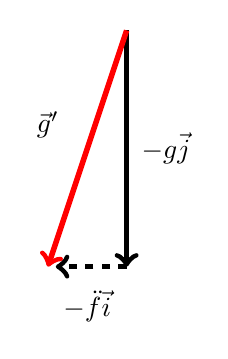
\begin{tikzpicture}
        \draw[->, line width=2] (0,0)--(0, -3);
        \draw[->, dashed, line width=2] (0, -3)--(-0.9, -3);
        \draw[->, red, line width=2] (0, 0)--(-1, -3);
        \node at (0.5, -1.5) {$-g\vec{j}$};
        \node at (-0.5, -3.5) {$-\ddot{f}\vec{i}$};
        \node at (-1, -1.2) {$\vec{g}^\prime$};
    \end{tikzpicture}
    \caption{Sketch of equivalent gravity $\vec{g}^\prime$}
    \label{Sketch of equivalent gravity}
\end{figure}

The system can be seen as a double pendulum that act under the equivalent gravity.

\subsection{A Case: Solution From Mathematica and Discussion}

Here gives a simple case, where $f(t)$ is as below:
\begin{equation}
    f(t)=\frac{3}{2}t^2 + t
\end{equation}

which means the acceleration of the frame is:
\begin{equation}
    a=\ddot{f} = 3m/s^2
\end{equation}

Other parameters are shown as follow:
\begin{itemize}
    \item $m_1=2kg$ , $m_2=1kg$;
    \item $g=9.8m/s^2$;
    \item $l_1=50cm$ , $l_2=30cm$.
\end{itemize}

and set the initial condition:
\begin{equation}
    \theta_1(0)=10^\circ\quad
    \theta_2(0)=20^\circ\quad
    \dot{\theta}_1(0)=2rad/s\quad
    \dot{\theta}_2(0)=1rad/s
\end{equation}

Using Mathematica's 'NDSolve' function to solve this ODE numerically. 
And the simulation time $t=0\sim 10s$. 
$\theta_1(t),\theta_2(t)$'s variation is plotted as follow:
\begin{figure}[H]
    \centering
    \includegraphics[width=0.7\textwidth]{..//problem2/angle.pdf}
    \caption{The variation $\theta_1$ and $\theta_2$ within time}
\end{figure}

The lines of $\theta_1$ and $\theta_2$ fluctuate around $-15\sim-20$, 
which is exactly:
\begin{equation}
    \alpha = -\arctan\frac{\ddot{f}}{g} = -\arctan\frac{3}{9.8}\approx -17.02^\circ
\end{equation}

Below is the figure at different time, of which the dashed line means the direction of 
equivalent gravity. 
These series figures illustrate that the prescribed motion $x=f(t)$ actually adds an extra 
acceleration to the two pendulum system. 
You can find all these pictures , vivid gif and Mathematica calculation notebook in path 'problem2'.
\begin{figure}[H]
    \centering
    \subfloat[$t=0.0s$]{
        \includegraphics[width = 0.3\textwidth]{..//problem2/some_step/0.pdf}
    }\quad
    \subfloat[$t=0.2s$]{
        \includegraphics[width = 0.3\textwidth]{..//problem2/some_step/1.pdf}
    }\\
    \subfloat[$t=0.4s$]{
        \includegraphics[width = 0.3\textwidth]{..//problem2/some_step/2.pdf}
    }\quad
    \subfloat[$t=0.6s$]{
        \includegraphics[width = 0.3\textwidth]{..//problem2/some_step/3.pdf}
    }\\
    \subfloat[$t=0.8s$]{
        \includegraphics[width = 0.3\textwidth]{..//problem2/some_step/4.pdf}
    }\quad
    \subfloat[$t=1.0s$]{
        \includegraphics[width = 0.3\textwidth]{..//problem2/some_step/5.pdf}
    }\\
    \subfloat[$t=1.2s$]{
        \includegraphics[width = 0.3\textwidth]{..//problem2/some_step/6.pdf}
    }\quad
    \subfloat[$t=1.4s$]{
        \includegraphics[width = 0.3\textwidth]{..//problem2/some_step/7.pdf}
    }\\
    \subfloat[$t=1.6s$]{
        \includegraphics[width = 0.3\textwidth]{..//problem2/some_step/8.pdf}
    }\quad
    \subfloat[$t=1.8s$]{
        \includegraphics[width = 0.3\textwidth]{..//problem2/some_step/9.pdf}
    }
    \caption{Position of ths system at different time}
    \label{Position of ths system at different time}
\end{figure}